\documentclass[11pt,class=report,crop=false]{standalone}
\usepackage{exo7sv}

\begin{document}

%%%%%%%%%%%%%%%%%%%%%%%%%%%%%%%%%%%%%%%%%%%%%%%%%%%%%%%%%%%%%%%%%%%%%%
%%%%%%%%%%%%%%%%%%%%%%%%%%%%%%%%%%%%%%%%%%%%%%%%%%%%%%%%%%%%%%%%%%%%%%

\entete{Université de Lille}{Mathématiques pour la SVT}

\titre{Fiche 4. \quad \'Etude de fonctions} 

\encadre{
\emph{Savoir.}
\begin{itemize}[label=$\square$]
  \item Connaître les différentes étapes d'une étude de fonction.
  \item Connaître ses formules : fonctions usuelles, dérivées, limites.  
\end{itemize}
\emph{Savoir-faire.}
\begin{itemize}[label=$\square$]
	\item Savoir faire une étude complète de fonction.
	\item Savoir tracer le graphe d'une fonction.
    \item Savoir calculer les asymptotes.
\end{itemize}
}


On considère la fonction $f$ définie par l'expression $f(x)=\displaystyle\ln\bigg(\frac{x^2+1}{x}\bigg)$. Cet exemple servira de modèle pour expliquer comment réaliser une étude de fonction.

Les différentes étapes sont les suivantes (qu'il faudra éventuellement adapter selon la fonction).
\begin{enumerate}[label=\arabic*.]
  \item Domaine de définition
  \item Calcul de la dérivée
  \item Calcul des limites
  \item Sens de variation
  \item Tableau de variations
  \item Représentation graphique
  \item Asymptotes
\end{enumerate}

%%%%%%%%%%%%%%%%%%%%%%%%%%%%%%%%%%%%%%%%%%%%%%%%%%%
\subsection*{1. Domaine de définition}

\emph{Trouver l'ensemble de définition $\mathcal{D}_f$ de $f$ c'est répondre à la question: "Pour quels réels $x$ l'expression $f(x)$ a-t-elle un sens?"}
\begin{itemize}
	\item On sait que la fraction $\displaystyle\frac{x^2+1}{x}$ est définie pour $x\in\Rr^{*}$ ($\Rr^{*}=\Rr\setminus\{0\}$).
	\item On sait que la fonction logarithme est définie sur $\Rr^{*}_{+}=]0,+\infty[$.
\end{itemize}
Il suffit donc de déterminer les réels non nuls $x$ tels que $\frac{x^2+1}{x}>0$.
Mais, comme $x^2+1>0$, cela équivaut à $x>0$ et donc $\mathcal{D}_f=\Rr^{*}_{+}=]0,+\infty[$.


\subsection*{2. Calcul des limites}

\emph{Pour une fonction $f$ donnée, on détermine ses limites sur la frontière de son ensemble de définition.}

Dans notre exemple $f(x)=\displaystyle\ln\bigg(\frac{x^2+1}{x}\bigg)$, on a montré que $\mathcal{D}_f=]0,+\infty[$. Ainsi, nous allons déterminer les limites de $f$  en $0$ (à droite) et en $+\infty$.

\textbf{Limite à droite en $0$.}
		\begin{itemize}
			\item On sait que $\lim\limits_{x\rightarrow 0^+}x^2+1=1$ et $\lim\limits_{x\rightarrow 0^+}x=0^+$ donc $\lim\limits_{x\rightarrow 0^+}\displaystyle\frac{x^2+1}{x}=+\infty$.
			\item On sait que $\lim\limits_{y\rightarrow +\infty}\ln(y)=+\infty$.
		\end{itemize}
		Ainsi, $\lim\limits_{x\rightarrow 0^+}\displaystyle\ln\bigg(\frac{x^2+1}{x}\bigg)=+\infty$.

\newpage
\textbf{Limite en $+\infty$.}

		\begin{itemize}
			\item Pour tout $x>0$ on a: \[\frac{x^2+1}{x}=\frac{x^2\bigg(1+\frac{1}{x^2}\bigg)}{x}=x\bigg(1+\frac{1}{x^2}\bigg).\]
			\item On sait que $\lim\limits_{x\rightarrow +\infty}\displaystyle\frac{1}{x^2}=0$ et donc que $\lim\limits_{x\rightarrow +\infty}\displaystyle1+\frac{1}{x^2}=1$. D'où $\lim\limits_{x\rightarrow +\infty}\displaystyle\frac{x^2+1}{x}=+\infty$.
		\end{itemize}
		Ainsi, $\lim\limits_{x\rightarrow +\infty}\displaystyle\ln\bigg(\frac{x^2+1}{x}\bigg)=+\infty$.

\subsection*{3. Calcul de la dérivée}

La fonction $f$ est dérivable sur $]0,+\infty[$, calculons sa dérivée $f'$.

\begin{itemize}
	\item On sait que $f$ est de la forme $f(x)=\ln(u(x))$ avec $u(x)=\displaystyle \frac{x^2+1}{x}$. Donc, pour tout $x>0$, on a: $f'(x)=\displaystyle \frac{u'(x)}{u(x)}$. 
	\item On sait que $u$ est de la forme $u(x)=\displaystyle \frac{v(x)}{w(x)}$ avec $v(x)=x^2+1$ et $w(x)=x$. Donc, pour tout $x>0$, on a: $u'(x)=\displaystyle \frac{v'(x)w(x)-v(x)w'(x)}{(w(x))^2}$.
	\item On sait que $v'(x)=2x$ et $w'(x)=1$. Ainsi,  $u'(x)=\displaystyle \frac{2x^2-(x^2+1)}{x^2}=\frac{x^2-1}{x^2}$.
\end{itemize}
On peut donc conclure que, pour tout $x>0$, on a:
\[f'(x)=\frac{\frac{x^2-1}{x^2}}{\frac{x^2+1}{x}}=\frac{x^2-1}{x^2}\times\frac{x}{x^2+1}=\frac{x^2-1}{x(x^2+1)}.\]

\subsection*{4. Sens de variation}

\emph{Le signe de la dérivée d'une fonction permet de déterminer son sens de variation.}

\mybox{
\emph{Rappel.} Soit $I$ un intervalle et $f : I \to\Rr$ une fonction dérivable.
			 
\begin{enumerate}
	\item Si $f'(x)>0$ pour tout $x\in I$ alors $f$ est strictement croissante sur $I$.
	\item Si $f'(x)<0$ pour tout $x\in I$ alors $f$ est strictement décroissante sur $I$.
	\item Si $f'(x)=0$ pour tout $x\in I$ alors $f$ est constante sur $I$.
\end{enumerate}}

Dans notre exemple, commençons par déterminer le signe de $f'$. On sait que, pour tout $x>0$, on a: $f'(x)=\displaystyle\frac{x^2-1}{x(x^2+1)}$. Or, pour tout $x>0$, on a $x(x^2+1)>0$. Ainsi, le signe de $f'$ ne dépend que de celui de $x^2-1$ pour $x\in\Rr^{*}_{+}$. 

Déterminons le signe de $x^2-1$ : comme $x^2-1=(x-1)(x+1)$ (nous utilisons l'identité remarquable $a^2-b^2=(a-b)(a+b)$ avec $a=x$ et $b=1$) alors
$x^2-1<0$ pour tout $x\in]-1,1[$ et $x^2-1>0$ pour tout $x\in]-\infty,-1[\cup]1,+\infty[$.
Ainsi, 
\begin{itemize}
	\item on obtient: $f'(x)<0$ pour tout $x\in]0,1[$,
	\item on obtient: $f'(x)>0$ pour tout $x\in]1,+\infty[$,
	\item et $f'(1)=0$.
\end{itemize}
D'où:
\begin{itemize}
	\item La fonction $f$ est strictement décroissante sur $]0,1[$,
	\item La fonction $f$ est strictement croissante sur $]1,+\infty[$.
	\item le graphe de la fonction $f$ admet une tangente horizontale en $1$.
\end{itemize}


\subsection*{5. Tableau de variations}

\emph{Le tableau de variations permet de récapituler toutes les informations précédemment trouvées sur la fonction à étudier.}

 Dans le cas de la fonction définie par $f(x)=\displaystyle\ln\bigg(\frac{x^2+1}{x}\bigg)$, voici le tableau de variations que l'on obtient.
\[\begin{tabvar}{|C|CRCCCC|} 
\hline x   &0       & & &1         & &+\infty\\ \hline f'(x)&  \dbarre & &-&\barre{0} &+&\\ 
\hline \niveau{2}{2}\TVcenter{f(x)}&\dbarre &\niveau{2}{2}+\infty &\decroit&\barre{\ln(2)}&\croit&+\infty\\ \hline\end{tabvar}\]

On obtient également que $f$ admet un minimum local, qui est ici global, en $x=1$. Ce minimum global vaut $f(1)=\displaystyle\ln\bigg(\frac{1^2+1}{1}\bigg)=\ln(2)$.

\subsection*{6. Représentation graphique}

\emph{Le graphe d'une fonction est obtenu à partir des informations contenues dans le tableau de variation et du calcul de quelques valeurs.}

 
Voici la représentation graphique de la fonction $f$ définie par $f(x)=\displaystyle\ln\bigg(\frac{x^2+1}{x}\bigg)$.

	\begin{center}
		\begin{tikzpicture}[scale=1.5]
     		 \draw[->,>=latex, gray] (0,0)--(7.5,0) node[below,black] {$x$};
     		 \foreach\x in{0,2,3,4,5,6}{	\draw[very thick, gray] (\x,2pt) -- (\x,-2pt)node[below,gray] {\small$\x$};}
		     \draw[->,>=latex, gray] (0,0)--(0,5) node[left,black] {$y$};
       		 \foreach\y in{1,...,4}{	\draw[very thick, gray] (2pt,\y) -- (-2pt,\y)node[left,gray] {\small$\y$};}
		     \draw[ultra thick, color=red,domain=0.01:7,samples=100,smooth] plot (\x,{ln((\x^2+1)/\x)}) node[above]{$f(x)=\ln\left(\frac{x^2+1}{x}\right)$};
			 \fill (0,0) circle (2pt) node[below left]{$0$};
		     \fill (1,0) circle (2pt) node[below]{$1$};
		     \fill (0,0.693) circle (2pt) node[left]{$\ln(2)$};
		     \fill (1,0.693) circle (2pt);
		     \draw[dashed](1,0) -- (1,0.693) -- (0,0.693);
		\end{tikzpicture}
	\end{center}	


\newpage\subsection*{7. Asymptotes}

De gauche à droite : asymptote verticale, horizontale, oblique.
\begin{center}
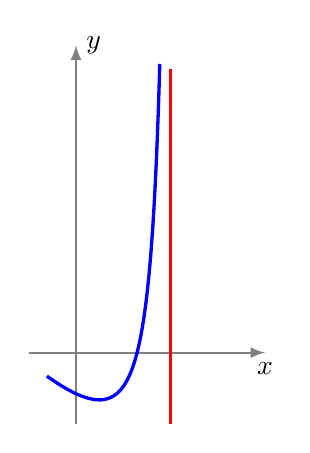
\begin{tikzpicture}[scale=0.6]
     \draw[->,>=latex,thick, gray] (-1,0)--(4,0) node[below,black] {$x$};
     \draw[->,>=latex,thick, gray] (0,-1.5)--(0,6.5) node[right,black] {$y$};

\begin{scope}[xshift=2cm, yshift=-3cm,rotate=90]
     \draw[very thick, red] (1.5,0)--(9,0);
     \draw [very thick, color=blue,samples=100,smooth, domain=1.5:10]
plot({\x-1+1/(\x-1)},{-0.2+1/(\x-1)+1/sqrt(\x))});
\end{scope}
  %  \fill (0,0) circle (1pt) node[above left] {$O$};
\end{tikzpicture}
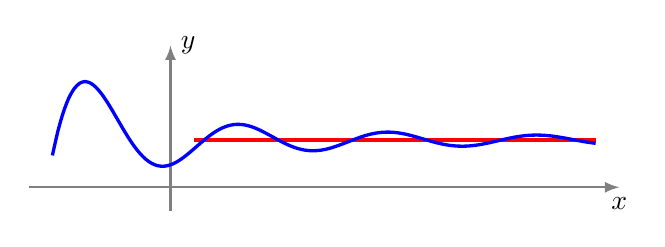
\begin{tikzpicture}[scale=0.6]
     \draw[->,>=latex,thick, gray] (-3,0)--(9.5,0) node[below,black] {$x$};
     \draw[->,>=latex,thick, gray] (0,-0.5)--(0,3) node[right,black] {$y$};

     \draw[very thick, red] (0.5,1)--(9,1);

     \draw [very thick, color=blue,samples=100,smooth, domain=1.5:13]
plot({-4+\x},{1-6*sin(2*\x r)*1/(\x*sqrt(2*\x))});

  %  \fill (0,0) circle (1pt) node[above left] {$O$};
\end{tikzpicture}
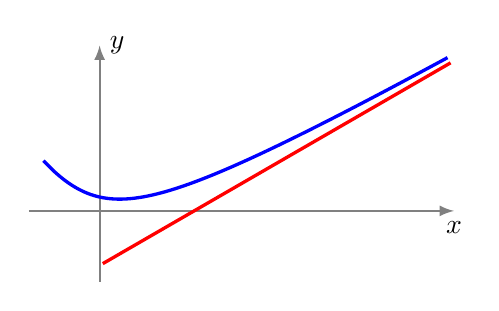
\begin{tikzpicture}[scale=0.6]
     \draw[->,>=latex,thick, gray] (-1.5,0)--(7.5,0) node[below,black] {$x$};
     \draw[->,>=latex,thick, gray] (0,-1.5)--(0,3.5) node[right,black] {$y$};

\begin{scope}[rotate=30, xshift=-1cm, yshift=-1cm]
     \draw[very thick, red] (0.5,0)--(9,0);
     \draw [very thick, color=blue,samples=100,smooth, domain=1.5:10]
plot({\x-1},{-0.3+1/(\x-1)+1/sqrt(\x))});
\end{scope}
  %  \fill (0,0) circle (1pt) node[above left] {$O$};
\end{tikzpicture}
\end{center}


\begin{itemize} 
  \item \textbf{Asymptote verticale.}
  Si, quand $x$ tend vers $a$, $f(x)$ tend vers $+\infty$ (ou
$-\infty$) la droite d'équation
$x=a$ est \emph{asymptote verticale} au graphe de $f$.

\item \textbf{Asymptote horizontale.} Si, quand $x$ tend vers $+\infty$, $f(x)$ tend vers $\ell \in \Rr$, la droite d'équation $y=\ell$ est \emph{asymptote horizontale} au graphe de $f$. 

\item \textbf{Asymptote oblique.}
La droite d'équation $y=ax+b$ est \emph{asymptote oblique} au graphe de $f$ :
\begin{enumerate}
  \item si $\frac{f(x)}{x}$ tend vers un réel $a$,
  \item et si $f(x)-ax$ tend vers un réel $b$.
\end{enumerate}
\end{itemize}

Pour l'exemple utilisé dans cette fiche, le graphe de $f$ admet une asymptote verticale en $0^+$. Des exemples d'asymptotes obliques seront faits en exercices.


\end{document}